\textbf{\LARGE{\color{tumgadPurple}AVL Trees}}\\
\\
\noindent
Given the following \href{https://sebastianoner.github.io/TUMGAD/src/DataStructures/SearchStructures/AVLTrees/AVLTrees}{\underline{AVL Tree}}:
%$INITTREE$
Perform the following operations in their given order on the tree above and check the boxes above the preprints
if any rotation was performed.
\begin{center}
    Insert: $FIRSTINSERTS$\\
    Delete: $DELETIONS$\\
    Insert: $SECONDINSERTS$\\
\end{center}
Insert: \underline{\hspace{.8cm}}
\hspace{.1cm}
\makebox[2.3cm][l]{$\square$ l rotation}
\makebox[2.3cm][l]{$\square$ r rotation}
\makebox[2.5cm][l]{$\square$ l-r rotation}
\makebox[2.5cm][l]{$\square$ r-l rotation}
\makebox[2.3cm][l]{$\square$ no rotation}
\begin{center}
    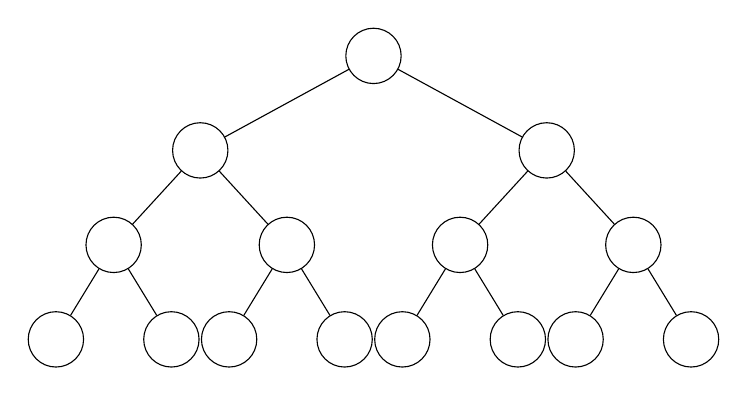
\begin{tikzpicture}[level/.style={sibling distance=55mm/#1},minimum size=25pt,scale=0.8,
    every node/.style={transform shape}]
        \node[circle,draw](z){}
        child{node[circle,draw]{}
            child{node[circle,draw]{}
                child{node[circle,draw]{}
                    child[missing]{}
                    child[missing]{}}
                child{node[circle,draw]{}
                    child[missing]{}
                    child[missing]{}}}
            child{node[circle,draw]{}
                child{node[circle,draw]{}
                    child[missing]{}
                    child[missing]{}}
                child{node[circle,draw]{}
                    child[missing]{}
                    child[missing]{}}}}
        child{node[circle,draw]{}
            child{node[circle,draw]{}
                child{node[circle,draw]{}
                    child[missing]{}
                    child[missing]{}}
                child{node[circle,draw]{}
                    child[missing]{}
                    child[missing]{}}}
            child{node[circle,draw]{}
                child{node[circle,draw]{}
                    child[missing]{}
                    child[missing]{}}
                child{node[circle,draw]{}
                    child[missing]{}
                    child[missing]{}}}};
    \end{tikzpicture}
\end{center}
Insert: \underline{\hspace{.8cm}}
\hspace{.1cm}
\makebox[2.3cm][l]{$\square$ l rotation}
\makebox[2.3cm][l]{$\square$ r rotation}
\makebox[2.5cm][l]{$\square$ l-r rotation}
\makebox[2.5cm][l]{$\square$ r-l rotation}
\makebox[2.3cm][l]{$\square$ no rotation}
\begin{center}
    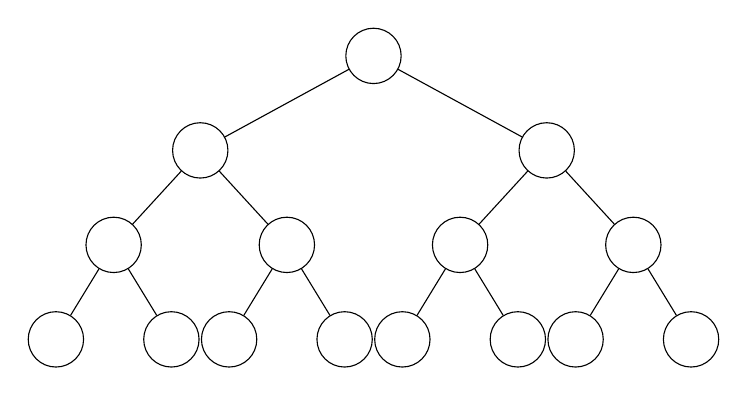
\begin{tikzpicture}[level/.style={sibling distance=55mm/#1},minimum size=25pt,scale=0.8,
    every node/.style={transform shape}]
        \node[circle,draw](z){}
        child{node[circle,draw]{}
            child{node[circle,draw]{}
                child{node[circle,draw]{}
                    child[missing]{}
                    child[missing]{}}
                child{node[circle,draw]{}
                    child[missing]{}
                    child[missing]{}}}
            child{node[circle,draw]{}
                child{node[circle,draw]{}
                    child[missing]{}
                    child[missing]{}}
                child{node[circle,draw]{}
                    child[missing]{}
                    child[missing]{}}}}
        child{node[circle,draw]{}
            child{node[circle,draw]{}
                child{node[circle,draw]{}
                    child[missing]{}
                    child[missing]{}}
                child{node[circle,draw]{}
                    child[missing]{}
                    child[missing]{}}}
            child{node[circle,draw]{}
                child{node[circle,draw]{}
                    child[missing]{}
                    child[missing]{}}
                child{node[circle,draw]{}
                    child[missing]{}
                    child[missing]{}}}};
    \end{tikzpicture}
\end{center}
\newpage
\noindent
Insert: \underline{\hspace{.8cm}}
\hspace{.1cm}
\makebox[2.3cm][l]{$\square$ l rotation}
\makebox[2.3cm][l]{$\square$ r rotation}
\makebox[2.5cm][l]{$\square$ l-r rotation}
\makebox[2.5cm][l]{$\square$ r-l rotation}
\makebox[2.3cm][l]{$\square$ no rotation}
\begin{center}
    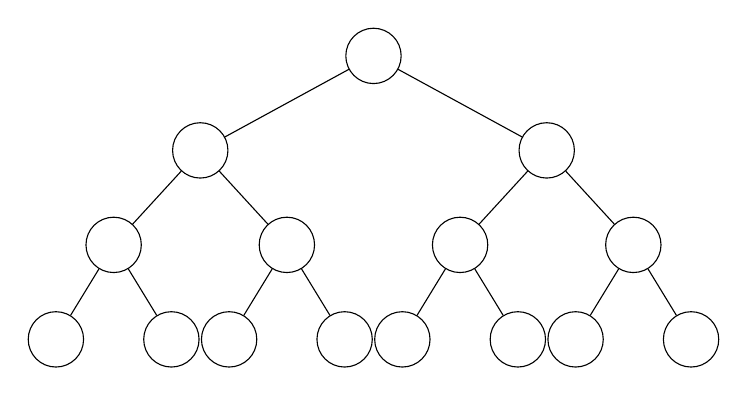
\begin{tikzpicture}[level/.style={sibling distance=55mm/#1},minimum size=25pt,scale=0.8,
    every node/.style={transform shape}]
        \node[circle,draw](z){}
        child{node[circle,draw]{}
            child{node[circle,draw]{}
                child{node[circle,draw]{}
                    child[missing]{}
                    child[missing]{}}
                child{node[circle,draw]{}
                    child[missing]{}
                    child[missing]{}}}
            child{node[circle,draw]{}
                child{node[circle,draw]{}
                    child[missing]{}
                    child[missing]{}}
                child{node[circle,draw]{}
                    child[missing]{}
                    child[missing]{}}}}
        child{node[circle,draw]{}
            child{node[circle,draw]{}
                child{node[circle,draw]{}
                    child[missing]{}
                    child[missing]{}}
                child{node[circle,draw]{}
                    child[missing]{}
                    child[missing]{}}}
            child{node[circle,draw]{}
                child{node[circle,draw]{}
                    child[missing]{}
                    child[missing]{}}
                child{node[circle,draw]{}
                    child[missing]{}
                    child[missing]{}}}};
    \end{tikzpicture}
\end{center}
Insert: \underline{\hspace{.8cm}}
\hspace{.1cm}
\makebox[2.3cm][l]{$\square$ l rotation}
\makebox[2.3cm][l]{$\square$ r rotation}
\makebox[2.5cm][l]{$\square$ l-r rotation}
\makebox[2.5cm][l]{$\square$ r-l rotation}
\makebox[2.3cm][l]{$\square$ no rotation}
\begin{center}
    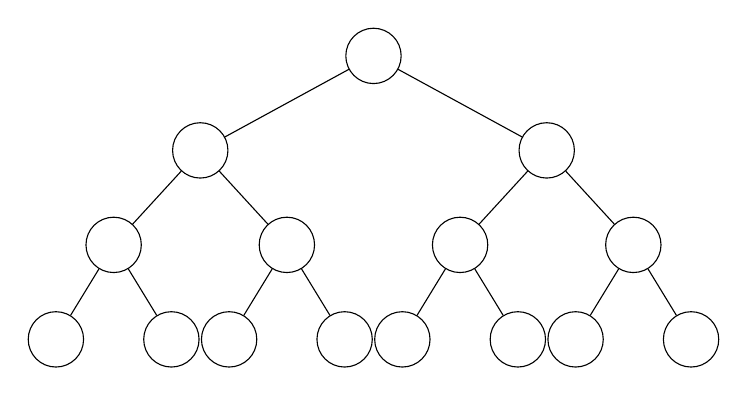
\begin{tikzpicture}[level/.style={sibling distance=55mm/#1},minimum size=25pt,scale=0.8,
    every node/.style={transform shape}]
        \node[circle,draw](z){}
        child{node[circle,draw]{}
            child{node[circle,draw]{}
                child{node[circle,draw]{}
                    child[missing]{}
                    child[missing]{}}
                child{node[circle,draw]{}
                    child[missing]{}
                    child[missing]{}}}
            child{node[circle,draw]{}
                child{node[circle,draw]{}
                    child[missing]{}
                    child[missing]{}}
                child{node[circle,draw]{}
                    child[missing]{}
                    child[missing]{}}}}
        child{node[circle,draw]{}
            child{node[circle,draw]{}
                child{node[circle,draw]{}
                    child[missing]{}
                    child[missing]{}}
                child{node[circle,draw]{}
                    child[missing]{}
                    child[missing]{}}}
            child{node[circle,draw]{}
                child{node[circle,draw]{}
                    child[missing]{}
                    child[missing]{}}
                child{node[circle,draw]{}
                    child[missing]{}
                    child[missing]{}}}};
    \end{tikzpicture}
\end{center}
Insert: \underline{\hspace{.8cm}}
\hspace{.1cm}
\makebox[2.3cm][l]{$\square$ l rotation}
\makebox[2.3cm][l]{$\square$ r rotation}
\makebox[2.5cm][l]{$\square$ l-r rotation}
\makebox[2.5cm][l]{$\square$ r-l rotation}
\makebox[2.3cm][l]{$\square$ no rotation}
\begin{center}
    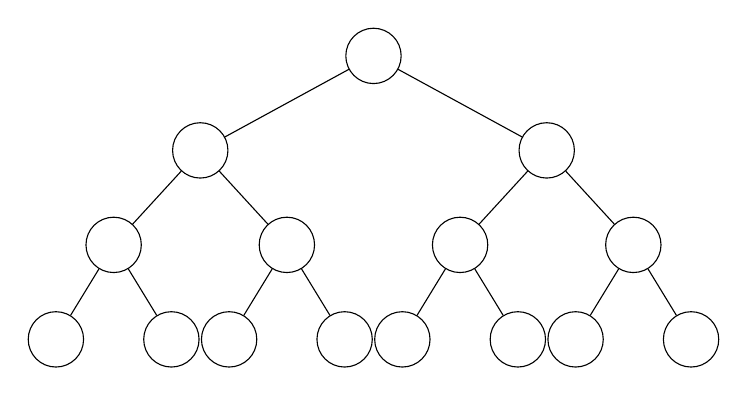
\begin{tikzpicture}[level/.style={sibling distance=55mm/#1},minimum size=25pt,scale=0.8,
    every node/.style={transform shape}]
        \node[circle,draw](z){}
        child{node[circle,draw]{}
            child{node[circle,draw]{}
                child{node[circle,draw]{}
                    child[missing]{}
                    child[missing]{}}
                child{node[circle,draw]{}
                    child[missing]{}
                    child[missing]{}}}
            child{node[circle,draw]{}
                child{node[circle,draw]{}
                    child[missing]{}
                    child[missing]{}}
                child{node[circle,draw]{}
                    child[missing]{}
                    child[missing]{}}}}
        child{node[circle,draw]{}
            child{node[circle,draw]{}
                child{node[circle,draw]{}
                    child[missing]{}
                    child[missing]{}}
                child{node[circle,draw]{}
                    child[missing]{}
                    child[missing]{}}}
            child{node[circle,draw]{}
                child{node[circle,draw]{}
                    child[missing]{}
                    child[missing]{}}
                child{node[circle,draw]{}
                    child[missing]{}
                    child[missing]{}}}};
    \end{tikzpicture}
\end{center}
Delete: \underline{\hspace{.8cm}}
\hspace{.1cm}
\makebox[2.3cm][l]{$\square$ l rotation}
\makebox[2.3cm][l]{$\square$ r rotation}
\makebox[2.5cm][l]{$\square$ l-r rotation}
\makebox[2.5cm][l]{$\square$ r-l rotation}
\makebox[2.3cm][l]{$\square$ no rotation}
\begin{center}
    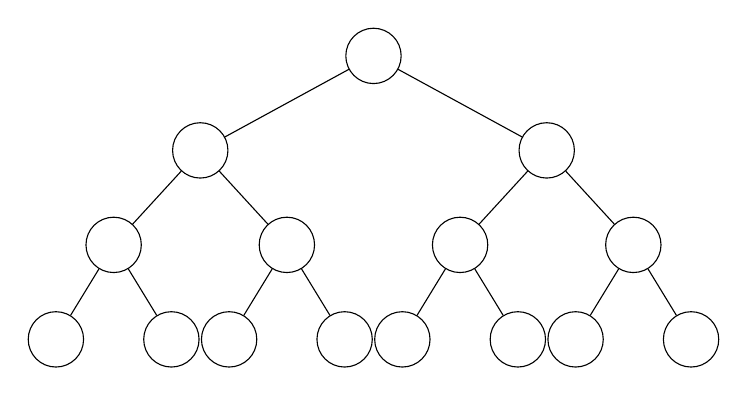
\begin{tikzpicture}[level/.style={sibling distance=55mm/#1},minimum size=25pt,scale=0.8,
    every node/.style={transform shape}]
        \node[circle,draw](z){}
        child{node[circle,draw]{}
            child{node[circle,draw]{}
                child{node[circle,draw]{}
                    child[missing]{}
                    child[missing]{}}
                child{node[circle,draw]{}
                    child[missing]{}
                    child[missing]{}}}
            child{node[circle,draw]{}
                child{node[circle,draw]{}
                    child[missing]{}
                    child[missing]{}}
                child{node[circle,draw]{}
                    child[missing]{}
                    child[missing]{}}}}
        child{node[circle,draw]{}
            child{node[circle,draw]{}
                child{node[circle,draw]{}
                    child[missing]{}
                    child[missing]{}}
                child{node[circle,draw]{}
                    child[missing]{}
                    child[missing]{}}}
            child{node[circle,draw]{}
                child{node[circle,draw]{}
                    child[missing]{}
                    child[missing]{}}
                child{node[circle,draw]{}
                    child[missing]{}
                    child[missing]{}}}};
    \end{tikzpicture}
\end{center}
\newpage
\noindent
Delete: \underline{\hspace{.8cm}}
\hspace{.1cm}
\makebox[2.3cm][l]{$\square$ l rotation}
\makebox[2.3cm][l]{$\square$ r rotation}
\makebox[2.5cm][l]{$\square$ l-r rotation}
\makebox[2.5cm][l]{$\square$ r-l rotation}
\makebox[2.3cm][l]{$\square$ no rotation}
\begin{center}
    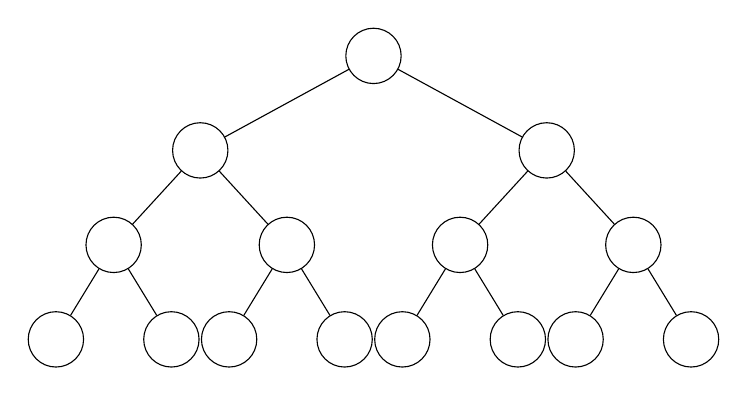
\begin{tikzpicture}[level/.style={sibling distance=55mm/#1},minimum size=25pt,scale=0.8,
    every node/.style={transform shape}]
        \node[circle,draw](z){}
        child{node[circle,draw]{}
            child{node[circle,draw]{}
                child{node[circle,draw]{}
                    child[missing]{}
                    child[missing]{}}
                child{node[circle,draw]{}
                    child[missing]{}
                    child[missing]{}}}
            child{node[circle,draw]{}
                child{node[circle,draw]{}
                    child[missing]{}
                    child[missing]{}}
                child{node[circle,draw]{}
                    child[missing]{}
                    child[missing]{}}}}
        child{node[circle,draw]{}
            child{node[circle,draw]{}
                child{node[circle,draw]{}
                    child[missing]{}
                    child[missing]{}}
                child{node[circle,draw]{}
                    child[missing]{}
                    child[missing]{}}}
            child{node[circle,draw]{}
                child{node[circle,draw]{}
                    child[missing]{}
                    child[missing]{}}
                child{node[circle,draw]{}
                    child[missing]{}
                    child[missing]{}}}};
    \end{tikzpicture}
\end{center}
Insert: \underline{\hspace{.8cm}}
\hspace{.1cm}
\makebox[2.3cm][l]{$\square$ l rotation}
\makebox[2.3cm][l]{$\square$ r rotation}
\makebox[2.5cm][l]{$\square$ l-r rotation}
\makebox[2.5cm][l]{$\square$ r-l rotation}
\makebox[2.3cm][l]{$\square$ no rotation}
\begin{center}
    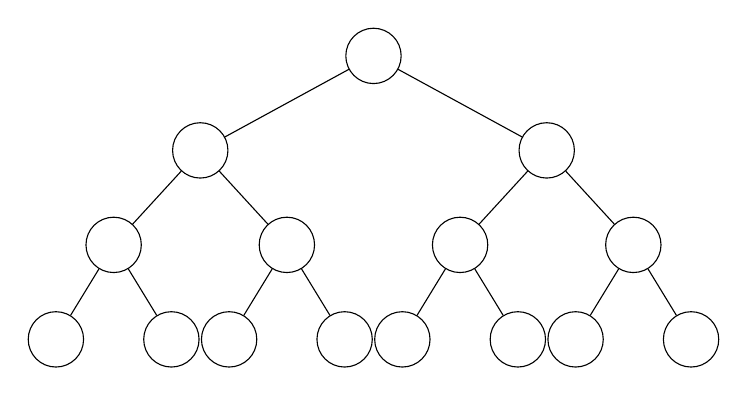
\begin{tikzpicture}[level/.style={sibling distance=55mm/#1},minimum size=25pt,scale=0.8,
    every node/.style={transform shape}]
        \node[circle,draw](z){}
        child{node[circle,draw]{}
            child{node[circle,draw]{}
                child{node[circle,draw]{}
                    child[missing]{}
                    child[missing]{}}
                child{node[circle,draw]{}
                    child[missing]{}
                    child[missing]{}}}
            child{node[circle,draw]{}
                child{node[circle,draw]{}
                    child[missing]{}
                    child[missing]{}}
                child{node[circle,draw]{}
                    child[missing]{}
                    child[missing]{}}}}
        child{node[circle,draw]{}
            child{node[circle,draw]{}
                child{node[circle,draw]{}
                    child[missing]{}
                    child[missing]{}}
                child{node[circle,draw]{}
                    child[missing]{}
                    child[missing]{}}}
            child{node[circle,draw]{}
                child{node[circle,draw]{}
                    child[missing]{}
                    child[missing]{}}
                child{node[circle,draw]{}
                    child[missing]{}
                    child[missing]{}}}};
    \end{tikzpicture}
\end{center}
Insert: \underline{\hspace{.8cm}}
\hspace{.1cm}
\makebox[2.3cm][l]{$\square$ l rotation}
\makebox[2.3cm][l]{$\square$ r rotation}
\makebox[2.5cm][l]{$\square$ l-r rotation}
\makebox[2.5cm][l]{$\square$ r-l rotation}
\makebox[2.3cm][l]{$\square$ no rotation}
\begin{center}
    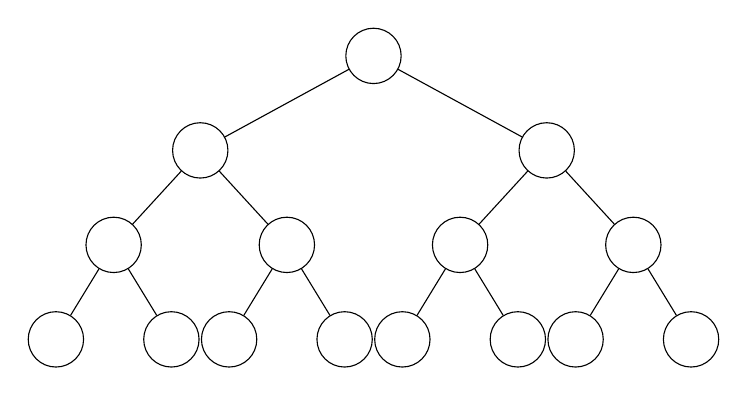
\begin{tikzpicture}[level/.style={sibling distance=55mm/#1},minimum size=25pt,scale=0.8,
    every node/.style={transform shape}]
        \node[circle,draw](z){}
        child{node[circle,draw]{}
            child{node[circle,draw]{}
                child{node[circle,draw]{}
                    child[missing]{}
                    child[missing]{}}
                child{node[circle,draw]{}
                    child[missing]{}
                    child[missing]{}}}
            child{node[circle,draw]{}
                child{node[circle,draw]{}
                    child[missing]{}
                    child[missing]{}}
                child{node[circle,draw]{}
                    child[missing]{}
                    child[missing]{}}}}
        child{node[circle,draw]{}
            child{node[circle,draw]{}
                child{node[circle,draw]{}
                    child[missing]{}
                    child[missing]{}}
                child{node[circle,draw]{}
                    child[missing]{}
                    child[missing]{}}}
            child{node[circle,draw]{}
                child{node[circle,draw]{}
                    child[missing]{}
                    child[missing]{}}
                child{node[circle,draw]{}
                    child[missing]{}
                    child[missing]{}}}};
    \end{tikzpicture}
\end{center}
Now give the $PRINTORDER$ visitation sequence of the AVL-Tree:\\
\\
\noindent\fbox{
    \parbox{\textwidth}{
        \vspace{0.6cm}
        \hspace{\textwidth}
    }
}
